\subsubsection{Navigation}
At first we tried to searching the panel by using long range laser sensor.
However, it was difficult to detect the panel because of the low density of points in long range.
So our second approach is running around the arena and searching the panel from pointcloud from the stereo camera.
When the panel is not visible within the robot's field of view, meaning that the panel is either out of range of the camera or is in another direction, the robot will naviagate around the arena to search for the panel.
Then when the panel enter the range of stereo camera, the robot recognizes the panel by finding
the cluster of pointcloud which places about 1 meter height from ground(Fig.\ref{fig: task2_panel-recognition}) and approach to the panel.
Finally, the robot runs around of the panel, recognizes it's the front side, then move to the front of the panel.

\begin{figure}[htb]
  \begin{center}
    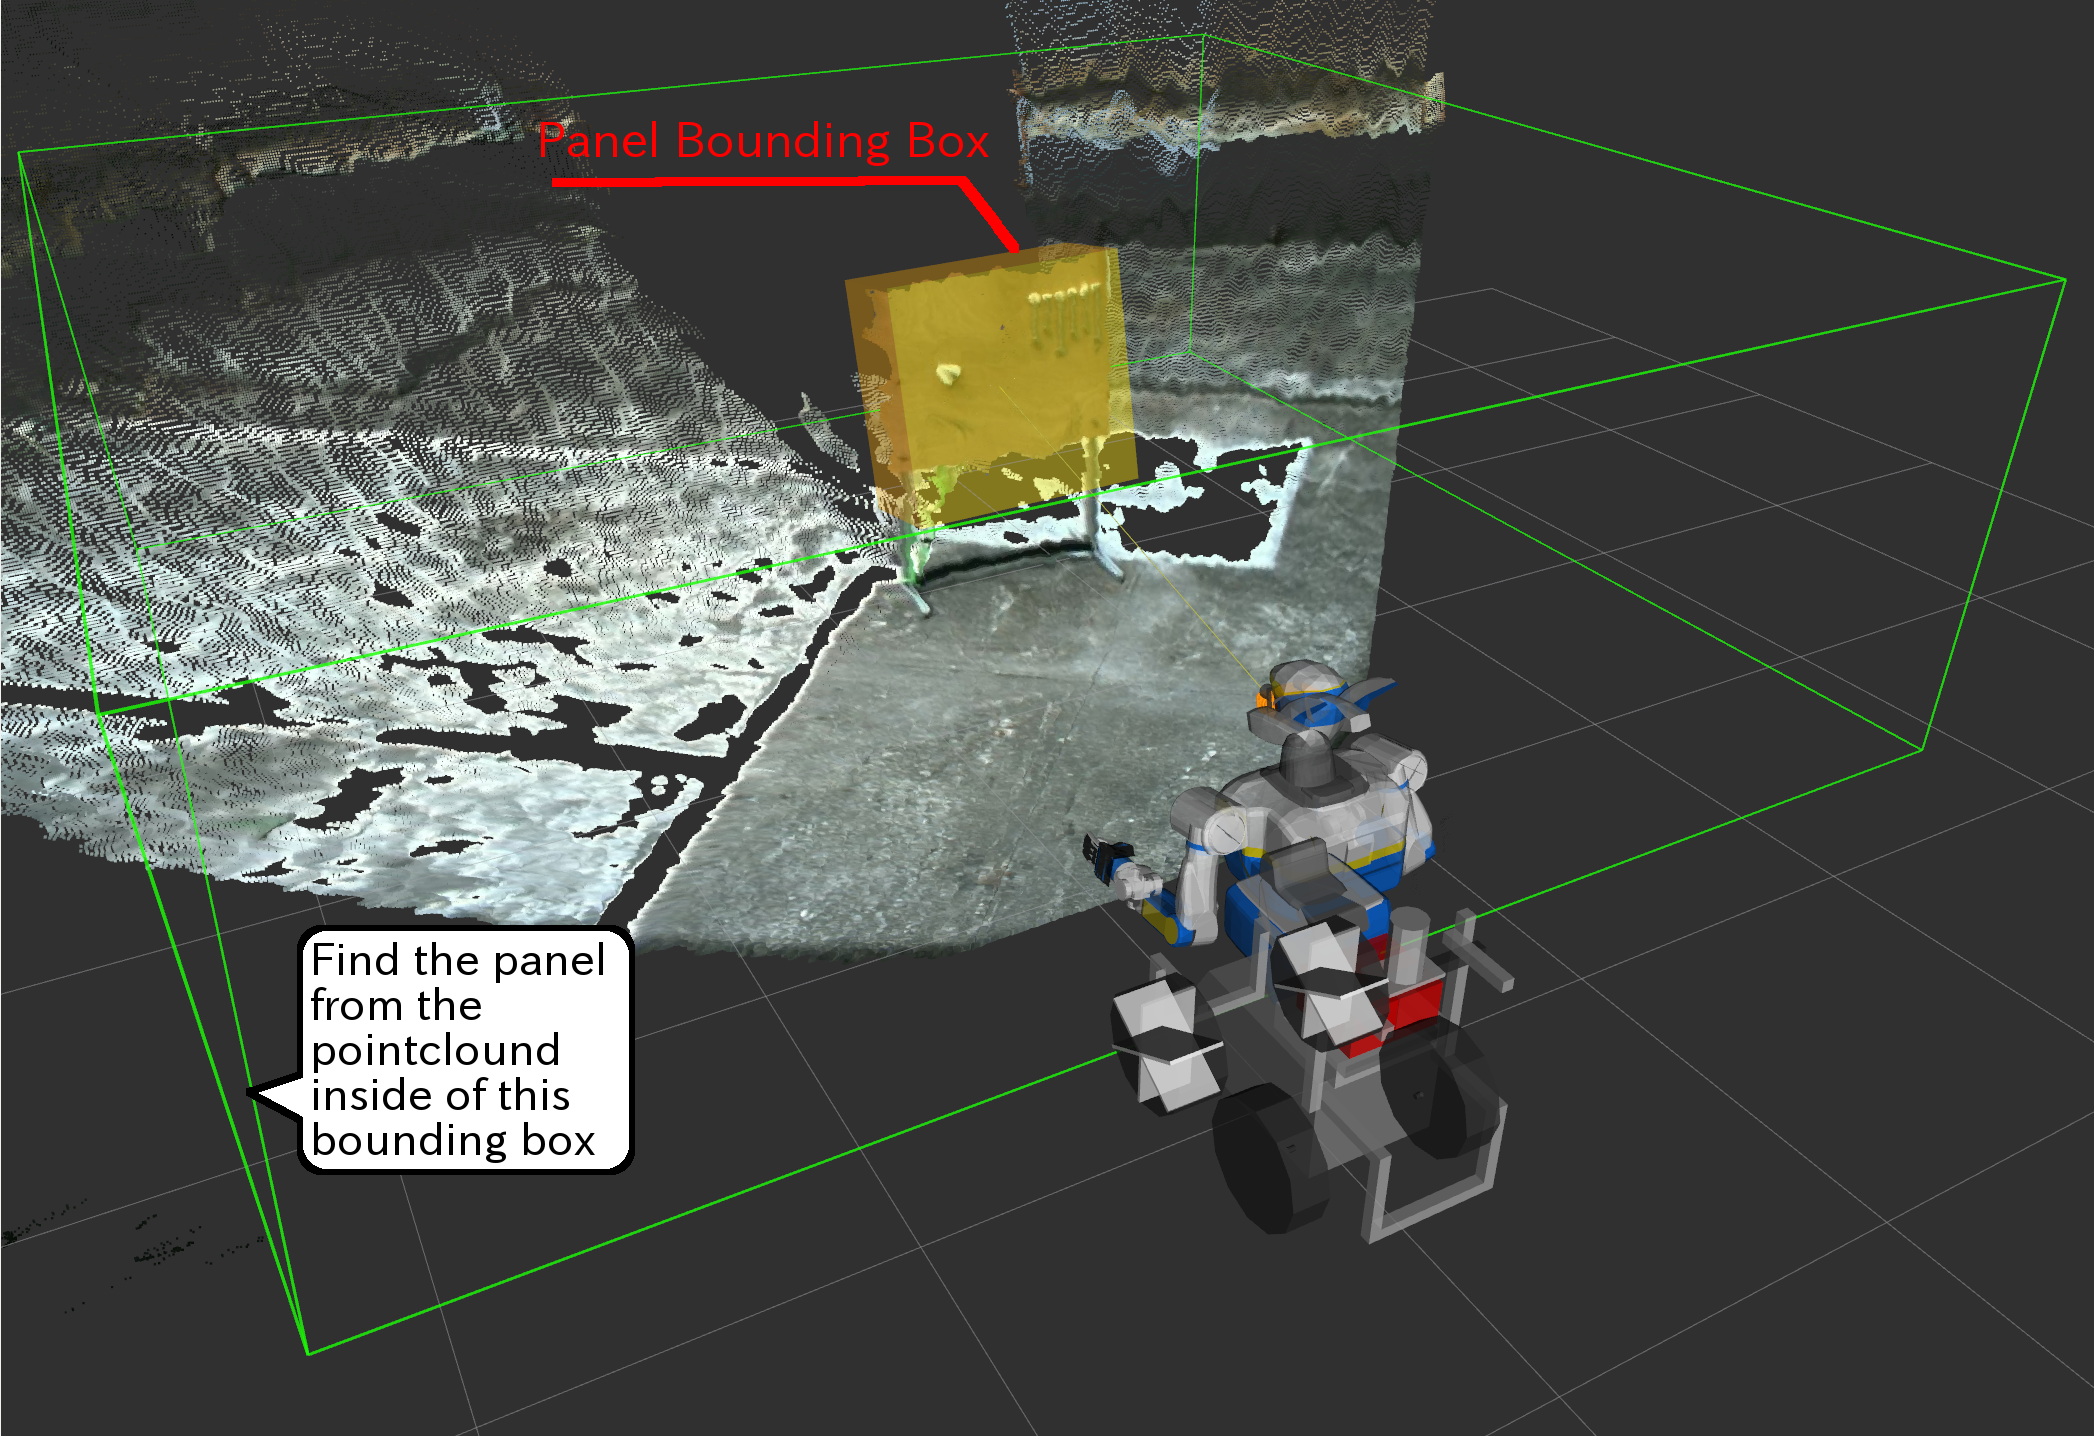
\includegraphics[width=0.80\columnwidth]{sections/task2/images/panel_detect.png}
    \caption{Panel Recognition from Pointcloud}
    \label{fig: task2_panel-recognition}
  \end{center}
\end{figure}

\subsubsection{Wrench and valve stem recognition}
We detected the wrenches and valve stem in manually selected ROI in previous report. We could recognize
the length of the wrenches and the position of the wrenches and valve stem.

Our next target is autonomous recognition and recognition of the rotation
of the panel relative to the robot.
We find the plane from pointclound which is in front of the robot, then find the upper-right corner of the panel and calcurate the rotation.
The transform of the wrenches and valve stem is fixed, so we can easily detect the position and rotation of them(Fig.\ref{fig: task2_object-recognition}).

We experimented our recognition method and confirmed the accuracy of the recognition is enough.

\begin{figure}[htb]
  \begin{center}
    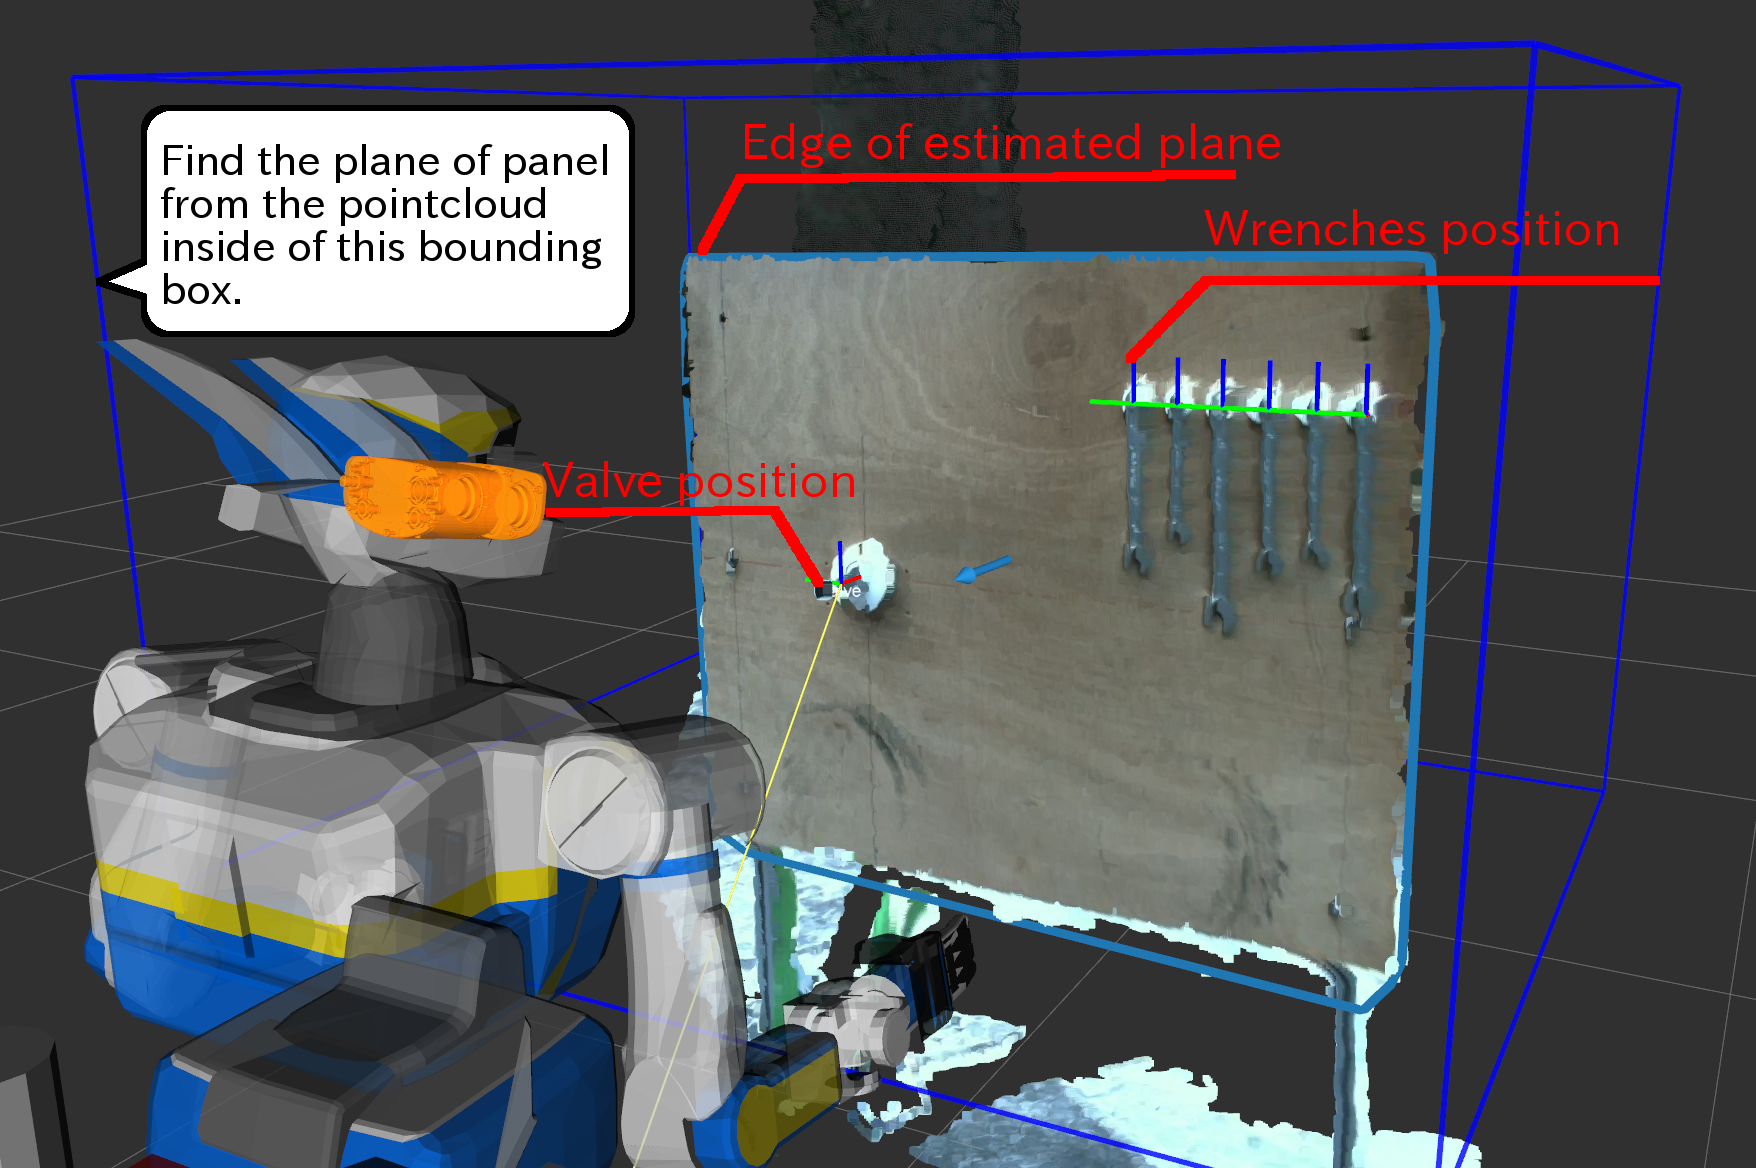
\includegraphics[width=0.80\columnwidth]{sections/task2/images/wrench_valve_recog.png}
    \caption{Wrenches and Valve Stem Recognition}
    \label{fig: task2_object-recognition}
  \end{center}
\end{figure}

\subsubsection{Picking the wrench}
We accomplished the wrench picking by just positioning the gripper to the detected wrench.

In order to improve the success rate, we are going to use handeye camera and image feedback control.


\subsubsection{Wrench fitting and turning}
We also accomplished wrench fitting and turning in previous report and are going to use handeye image feedback control.
